
\section{\stmt{ODER} Funktion}

$$ \text{\stmt{ODER( \syntax{Bedingung\_1}; \syntax{Bedingung\_2}; \ldots; \syntax{Bedingung\_255})}} $$

Die \stmt{ODER} Funktion gibt WAHR zurück wenn zumindest eine der Bedingungen WAHR ergibt.

\begin{description}[labelindent=0cm, leftmargin=3cm, font=\mdseries, labelwidth=3cm,style=nextline]
\item[Beispiele] \stmt{=ODER( 1<0 ; 8/4=2 )} $\Rightarrow$ WAHR \\
\stmt{=ODER( 1=2 ; 4/0,5=2 )} $\Rightarrow$ FALSCH
\end{description}
%
%
	\begin{figure}[H]
		\centering
%			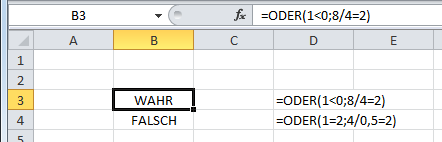
\includegraphics[width=11cm]{images/oder_1b}
			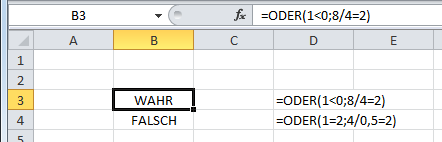
\includegraphics[scale=0.7]{images/oder_1b}
		\caption{\stmt{ODER} in einer Formel}
		\label{fig:oder}
	\end{figure}
